\section{Исследование сетей массового обслуживания}
\label{sec:part2}

\subsection{Исходные данные и граф модели M3}

В сети варианта \(41/3\) четыре узла с числом приборов
\(c=(3,2,1,1)\) и средним временем обслуживания
\(b=(4;2{,}5;14;5)\) с. Ёмкость очередей не ограничена. Заявки
в каждом узле обслуживаются в порядке поступления. Переходы между
узлами мгновенны.
После обслуживания в У1 заявка с равной вероятностью \(0{,}25\)
переходит в У2, У3, У4 или в точку 0. После периферийного узла она
всегда возвращается в У1. В замкнутой сети точка 0 отмечает конец
цикла и мгновенный вход в следующий цикл. В разомкнутой сети она
означает внешний источник на входе и сток на выходе.

\begin{figure}[htbp]
  \centering
  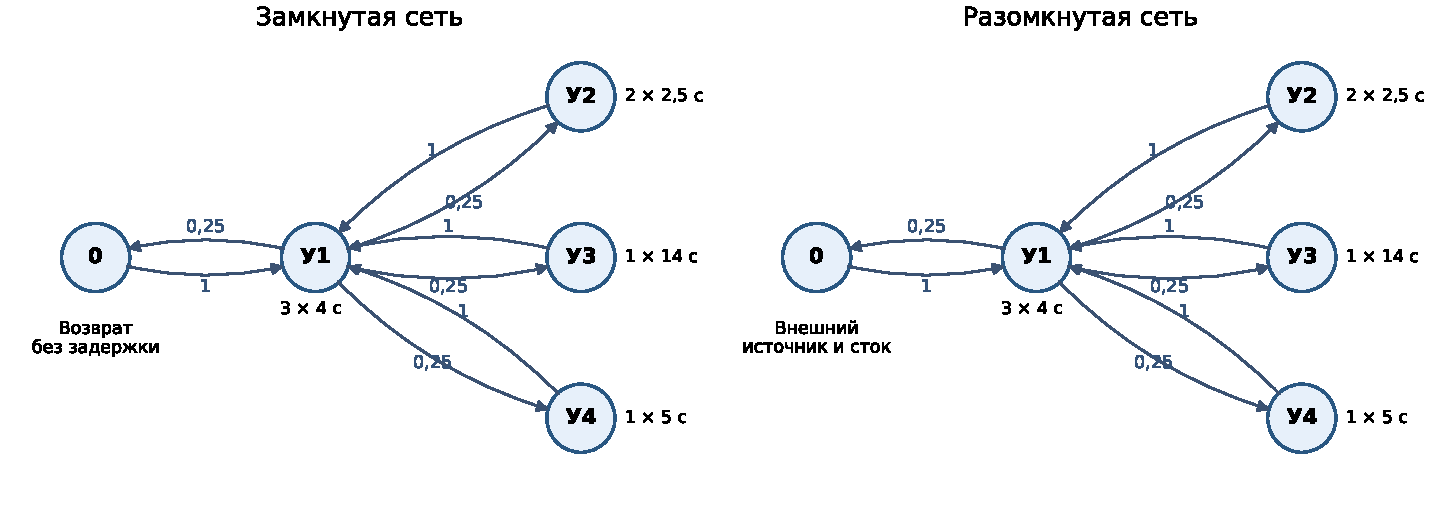
\includegraphics[width=\textwidth]{../out/part2/topology.pdf}
  \caption{Графы замкнутой и разомкнутой СеМО. В узлах указаны
  число приборов и средняя длительность обслуживания.}
  \label{fig:p2-network}
\end{figure}

При нормировке на выход одной заявки через точку 0 уравнения потоков
имеют вид
\[
  v_0=1,\qquad v_1=1+v_2+v_3+v_4,\qquad
  v_2=v_3=v_4=0{,}25v_1.
\]
Поэтому коэффициенты передач равны \(v=(4,1,1,1)\).
За цикл заявка в среднем проходит У1 четыре раза и по одному разу
посещает каждый периферийный узел. Суммарная потребность цикла в
обслуживании составляет \(\sum_i v_i b_i=37{,}5\) с. Потребность в
расчёте на один прибор составляет
\[
  \left(\frac{v_i b_i}{c_i}\right)_{i=1}^4
  = \left(\frac{16}{3};1{,}25;14;5\right)\ \text{с}.
\]
У3 ограничивает пропускную способность сети
\(X_{\max}=\min_i c_i/(v_i b_i)=1/14=0{,}071429\) заявки/с.
Для устойчивости разомкнутой сети нужно \(\lambda<X_{\max}\).
При \(\lambda=X_{\max}\) загрузка У3 достигает единицы, и конечное
стационарное среднее очереди к этому узлу отсутствует.

\subsection{GPSS-модель и план эксперимента}

Каждый узел использует последовательность блоков \texttt{QUEUE},
\texttt{ENTER}, \texttt{DEPART}, \texttt{ADVANCE}, \texttt{LEAVE}.
Ёмкость \texttt{STORAGE} равна числу одинаковых параллельных приборов.
После \texttt{MARK~2} значение \texttt{MP2} измеряет время с входа
в текущий узел. При входе в прибор это ожидание прибавляется к
параметру заявки, а после обслуживания по \texttt{MP2} измеряется
полное время посещения. В точке 0 \texttt{TABULATE} записывает
накопленное ожидание и длительность цикла либо пребывания заявки.
Маршрут из У1 выбирается по равномерному случайному числу из
1000 значений. Каждому из четырёх маршрутов соответствуют
250 значений. Из остальных узлов заявки возвращаются в У1.

В замкнутом варианте на старте создаётся \(M\) транзактов. В
разомкнутом варианте внешние заявки поступают через интервалы со
средним \(1/\lambda\), распределённые экспоненциально или заданные
постоянными. После прохождения У1 и выбора маршрута в точку 0
транзакт возвращается в замкнутую сеть или покидает разомкнутую.
Во всех опытах меняется одно указанное условие при сохранении
параметров базовой модели. Для исследования разброса времени
обслуживания меняется закон только в У2 при прежнем среднем
\(b_2=2{,}5\) с. Использованы экспоненциальное распределение,
\(E_2\) как сумма двух независимых экспоненциальных величин со
средним \(1{,}25\) с и гиперэкспоненциальное \(H_2\) с
коэффициентом вариации 2. В последнем случае выбирается одна из
двух экспоненциальных компонент с параметрами
\[
  p=\frac{1-\sqrt{3/5}}{2},\quad
  b_{21}=\frac{2{,}5}{2p},\quad b_{22}=\frac{2{,}5}{2(1-p)}.
\]
Обе компоненты вносят одинаковый вклад в общее среднее. Так
изменение длительности ожидания можно связать с разбросом
обслуживания и взаимодействием узлов.

Производительность \(X\) считали по числу завершённых циклов
или выходов за единицу времени. Чтобы сопоставить нагрузки, задавали
\(\lambda=X\) при одном и том же законе обслуживания в У2.
При фиксированном \(M\) проверили два способа разгрузить У3.
Среднее время обслуживания сокращали с 14 до 5 с или увеличивали
число приборов с одного до трёх. В обоих случаях наибольшая
потребность на прибор приходится на У1.

\subsection{Аналитическая проверка экспоненциальных моделей}

Для замкнутой сети с экспоненциальным обслуживанием рассчитаны
точные стационарные показатели. При состоянии
\(n=(n_1,\ldots,n_4)\), \(\sum_i n_i=M\), ненормированный вес равен
\[
  w(n)=\prod_{i=1}^4
      \frac{(v_i b_i)^{n_i}}{\prod_{j=1}^{n_i}\min(j,c_i)},\qquad
  G(M)=\sum_{\sum_i n_i=M}w(n),\qquad X(M)=\frac{G(M-1)}{G(M)}.
\]
Пустое произведение равно единице. Из сохранения популяции по
формуле Литтла среднее время цикла равно \(M/X(M)\). Для
разомкнутой экспоненциальной сети интенсивность в У\(i\) равна
\(\lambda v_i\), и ожидание в нём рассчитано по формуле Эрланга C
для \(M/M/c_i\). Сетевое ожидание — сумма узловых с весами \(v_i\).

Критическим считали наименьшее \(M\), при котором отставание
от предельной производительности \(1-X(M)/X_{\max}\) не превышает \(2\%\).
При \(M=5\) расчёт даёт \(X=0{,}068601\) заявки/с
(\(3{,}96\%\) до предела), при \(M=6\) — \(0{,}070167\) заявки/с
(\(1{,}77\%\)). Таким образом, \(M^*=6\).
Рост \(M\) сначала сокращает простой У3, поэтому растёт
производительность. Затем У3 почти всё время занят, новые заявки
в основном увеличивают очередь. При почти постоянном \(X\) среднее
время цикла \(M/X\) продолжает расти почти линейно. В разомкнутой
сети механизм иной: при приближении \(\lambda\) к \(1/14\) в У3
время ожидания растёт примерно как \(1/(1/14-\lambda)\), поскольку
внешний источник не ограничивает суммарное число заявок.

\subsection{Замкнутая сеть и устранение узкого места}

В основной серии GPSS World для каждой из 37 конфигураций сделали
по три прогона. Модель прогревали \(25\,000\) с, затем собирали
данные \(250\,000\) с. Начальные состояния генераторов меняли
между повторами. При сравнении конфигураций в одном повторе
их сохраняли, чтобы уменьшить вклад случайного разброса. На графиках
отрезки показывают одно стандартное отклонение по прогонам.

При \(M=5\) среднее измеренное \(X=0{,}069228\) заявки/с
на \(3{,}08\%\) ниже предела, при \(M=6\) значение
\(X=0{,}070864\) заявки/с находится на расстоянии \(0{,}79\%\)
от предела. Первый переход через уровень \(98\%\) предельной
производительности подтверждает \(M^*=6\). В этой точке среднее
время цикла составило \(84{,}66\) с, а по формуле Литтла с
измеренным \(X\) получается \(M/X=84{,}67\) с. Точный расчёт
для этой точки даёт \(X=0{,}070167\) заявки/с. Различие
с измерением составило \(0{,}99\%\). При \(M\geq7\) часть
конечных оценок \(X\) немного выше \(1/14\). Предельная
пропускная способность относится к установившемуся среднему,
тогда как в конкретной реализации длительности обслуживания
случайны.

\begin{figure}[htbp]
 \centering
 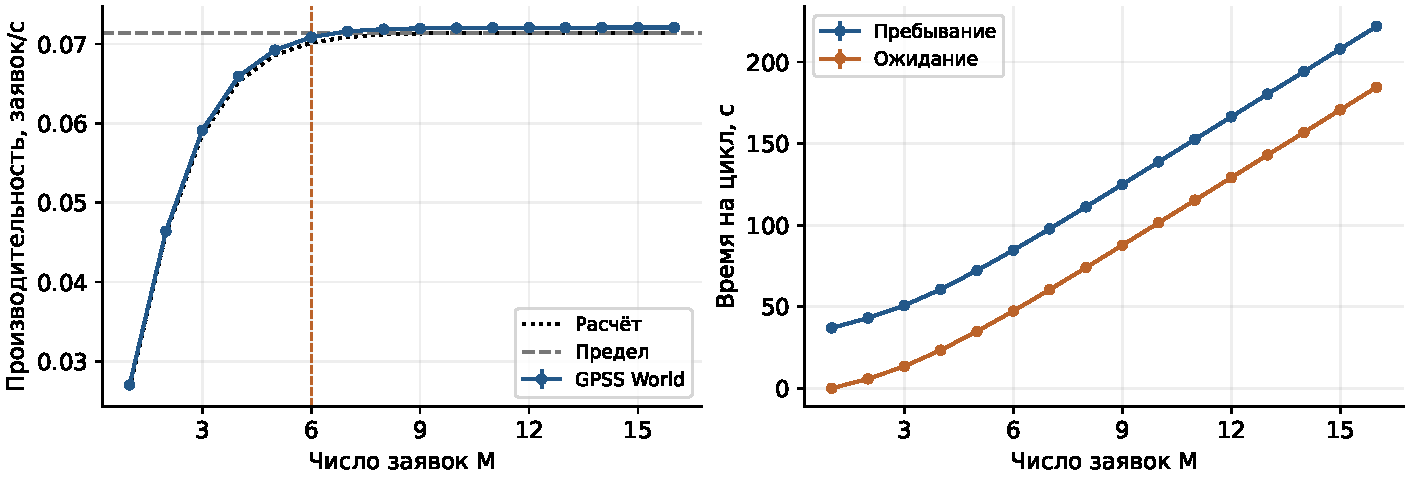
\includegraphics[width=\textwidth]{../out/part2/gpss/closed_scaling.pdf}
 \caption{Производительность и длительность цикла замкнутой сети}
 \label{fig:p2-scaling}
\end{figure}

\begin{table}[htbp]
 \centering
 \caption{Эффект устранения узкого места в замкнутой сети при \(M=6\)}
 \label{tab:p2-bottleneck}
 \begin{tabular}{@{}lrrrr@{}}
 \toprule
 Конфигурация & \(X\), заявок/с & \(\overline W\), с & \(\overline T\), с & \(\rho_3\) \\
 \midrule
 Исходная         & 0,07086 & 47,37 & 84,66 & 0,982\\
 \(b_3=5\) с      & 0,13646 & 15,55 & 43,96 & 0,677\\
 \(c_3=3\)        & 0,12952 &  8,98 & 46,32 & 0,599\\
 \bottomrule
 \end{tabular}
\end{table}

При уменьшении \(b_3\) или увеличении \(c_3\) производительность
выросла соответственно в \(1{,}93\) и \(1{,}83\) раза. Три
прибора У3 сильнее сокращают ожидание, но время пребывания
чуть выше, чем при \(b_3=5\) с. В конфигурации с тремя
приборами длительность обслуживания в У3 остаётся равной
\(14\) с. Оба изменения переносят ограничение в У1.
Предельная производительность становится равной
\(3/16=0{,}1875\) заявки/с.

При \(M=6\) смена закона в У2 почти не изменила среднее время
пребывания в сети. Оно составило \(84{,}66\) с для
экспоненциального закона, \(84{,}66\) с для \(E_2\) и
\(84{,}67\) с для \(H_2\). Стандартное отклонение по прогонам
намного больше разницы между этими средними. В самом У2 среднее
ожидание на тех же прогонах составляет \(0{,}0177\),
\(0{,}0159\) и \(0{,}0262\) с. У2 имеет два прибора
и низкую загрузку. Основное ожидание приходится на У3,
поэтому влияние формы распределения обслуживания лучше
видно в узловой статистике.

\begin{figure}[htbp]
 \centering
 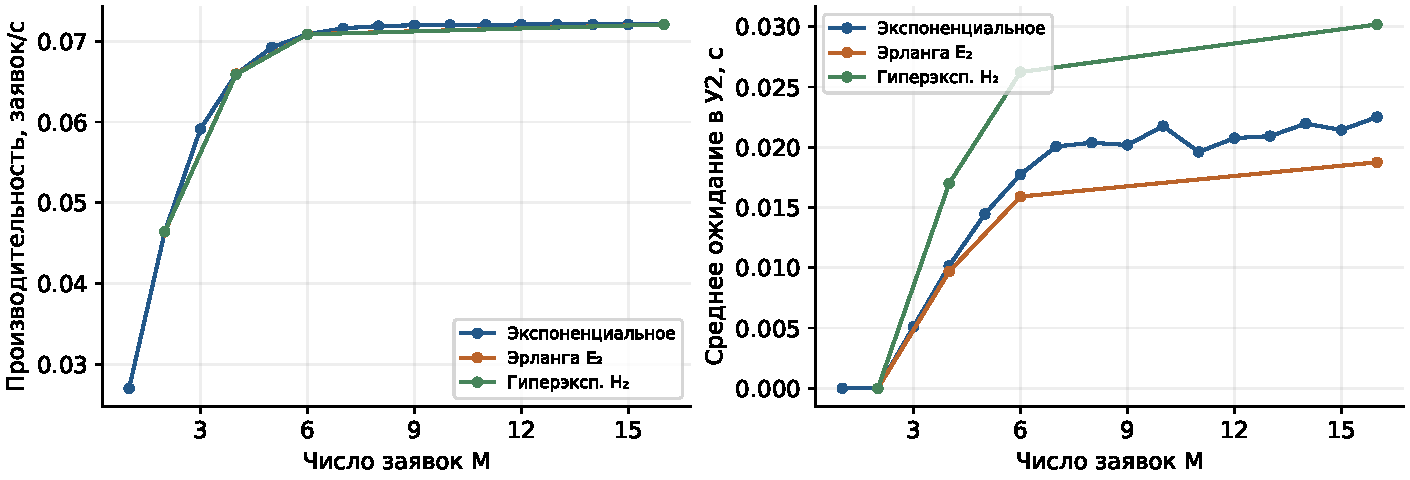
\includegraphics[width=\textwidth]{../out/part2/gpss/closed_service.pdf}
 \caption{Влияние закона обслуживания У2 при разных популяциях}
 \label{fig:p2-closed-service}
\end{figure}

\subsection{Разомкнутая сеть}

При простейшем внешнем потоке и экспоненциальном обслуживании
производительность в устойчивом режиме равна интенсивности
входа. При росте заданной нагрузки У3 с \(0{,}80\) до
\(0{,}95\) среднее пребывание увеличилось с \(90{,}37\) до
\(224{,}89\) с. Измеренная загрузка У3 выросла с \(0{,}777\)
до \(0{,}925\), а среднее число ожидающих в его очереди —
с \(2{,}86\) до \(12{,}38\). В верхней точке межпрогонное
стандартное отклонение времени пребывания составило
\(24{,}71\) с, оценка производительности — \(0{,}066915\)
заявки/с при заданных \(0{,}067857\) заявки/с. Точный расчёт при номинальной нагрузке
\(0{,}95\) даёт \(307{,}01\) с. В этой области среднее
ожидание чувствительно к изменению фактической загрузки,
поэтому даже небольшое отклонение входной производительности
и длительности обслуживания в отдельной реализации заметно
сказывается на оценке задержки.

\begin{figure}[htbp]
 \centering
 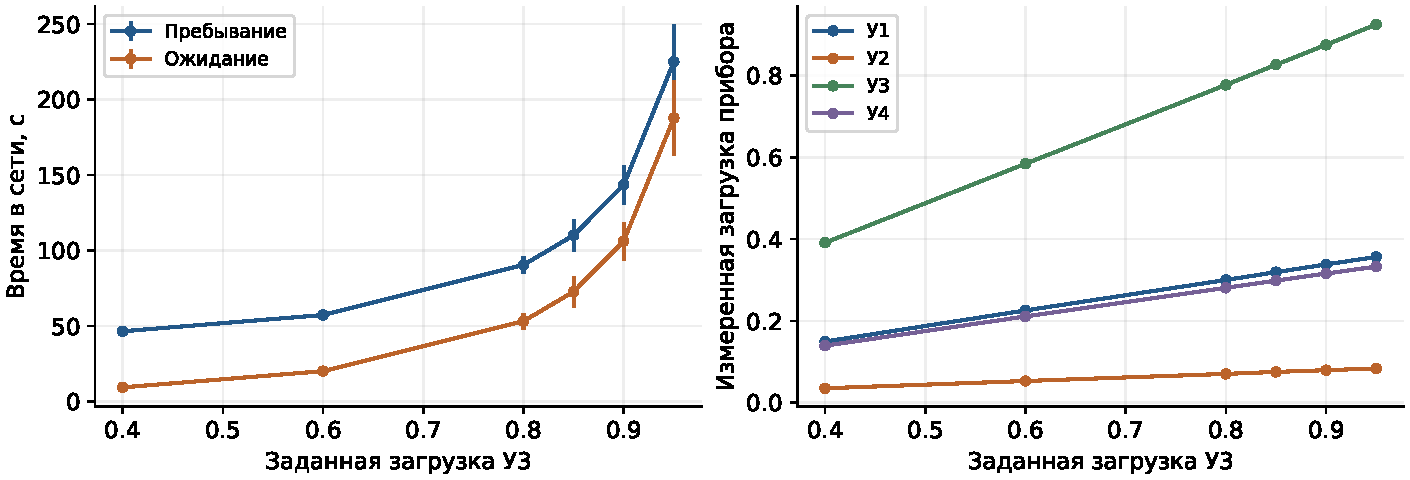
\includegraphics[width=\textwidth]{../out/part2/gpss/open_load.pdf}
 \caption{Задержки и загрузка узлов разомкнутой сети}
 \label{fig:p2-open}
\end{figure}

Законы обслуживания также сравнили при одной и той же заданной
нагрузке \(\rho_3=0{,}90\). При простейшем внешнем
потоке среднее ожидание в У2 составляет \(0{,}0173\),
\(0{,}0126\) и \(0{,}0263\) с для экспоненциального
обслуживания, \(E_2\) и \(H_2\). Коэффициент вариации
времени пребывания в У2 соответственно равен \(0{,}99\),
\(0{,}70\) и \(1{,}97\). С детерминированным внешним
потоком среднее ожидание в У2 составило \(0{,}0120\), \(0{,}0099\) и
\(0{,}0184\) с. При заданной интенсивности форма закона У2
практически не меняет загрузку У3. Замена внешнего потока
снизила среднее сетевое пребывание с \(143{,}42\) до
\(124{,}19\) с при экспоненциальном обслуживании. Изменение
сопоставимо с разбросом между повторами, поэтому вывод
относится к наблюдаемому эффекту в этих опытах.
Коэффициент вариации сетевого пребывания при простейшем
потоке практически одинаков для всех трёх законов У2
(\(1{,}85\)–\(1{,}87\)), с регулярным потоком он лежит
в диапазоне \(1{,}80\)–\(1{,}82\). Коэффициент вариации
сетевого ожидания для этих же конфигураций составлял
\(2{,}25\)–\(2{,}29\). Задержки в У3 определяют общий
разброс сильнее, чем изменение формы обслуживания в У2.

\subsection{Сопоставление сетей при равном потоке}

Для каждого закона обслуживания У2 измерили среднее \(X\)
замкнутой сети при \(M=6\) и задали такую же интенсивность входа
в разомкнутой модели. Заданная загрузка У3 получилась около
\(0{,}992\), поэтому прогрев увеличили до \(100\,000\) с,
а время наблюдения — до \(800\,000\) с. Для разомкнутой сети
проверили шесть конфигураций, по три прогона на каждую.
В таблице~\ref{tab:p2-matched} после знака \(\pm\) указаны
стандартные отклонения по повторам. Журнал завершённой серии
показан на рисунке~\ref{fig:gp-network-campaign}.

\begin{table}[htbp]
 \centering
 \caption{Среднее пребывание при совпадении интенсивности входа РСеМО
 и производительности ЗСеМО для каждого закона У2}
 \label{tab:p2-matched}
 \begin{tabular}{@{}lrrrr@{}}
 \toprule
 Закон У2 & \(\lambda\), заявок/с & ЗСеМО, с &
 \multicolumn{2}{c@{}}{РСеМО, с} \\
 \cmidrule(l){4-5}
 & & & Простейший поток & Регулярный поток \\
 \midrule
 Экспоненциальный & 0,070864 & 84,66 & \(1061{,}52\pm629{,}38\) & \(721{,}65\pm260{,}00\) \\
 \(E_2\)          & 0,070867 & 84,66 & \(1063{,}48\pm631{,}17\) & \(723{,}41\pm261{,}19\) \\
 \(H_2\)          & 0,070847 & 84,67 & \(1048{,}23\pm618{,}85\) & \(711{,}04\pm252{,}90\) \\
 \bottomrule
 \end{tabular}
\end{table}

Для экспоненциальной пары измеренная производительность
открытой сети с простейшим потоком составила \(0{,}070763\)
заявки/с, что на \(0{,}14\%\) ниже заданной интенсивности.
В разомкнутой сети среднее время пребывания больше
из-за накопления очереди в У3 при загрузке, близкой
к единице. В замкнутой сети общее число заявок
ограничено шестью. Регулярный внешний поток даёт
меньшие средние во всех трёх парах. При этом разброс
сетевого времени между прогонами велик, поэтому малые
различия между законами обслуживания У2 интерпретируются
по узловой статистике и по опытам при меньшей нагрузке.
Точный экспоненциальный расчёт при \(\lambda=0{,}070864\)
даёт \(1798{,}58\) с. Отличие от имитационной оценки
указывает на высокую неопределённость численного сравнения
вблизи границы устойчивости.

\begin{figure}[htbp]
 \centering
 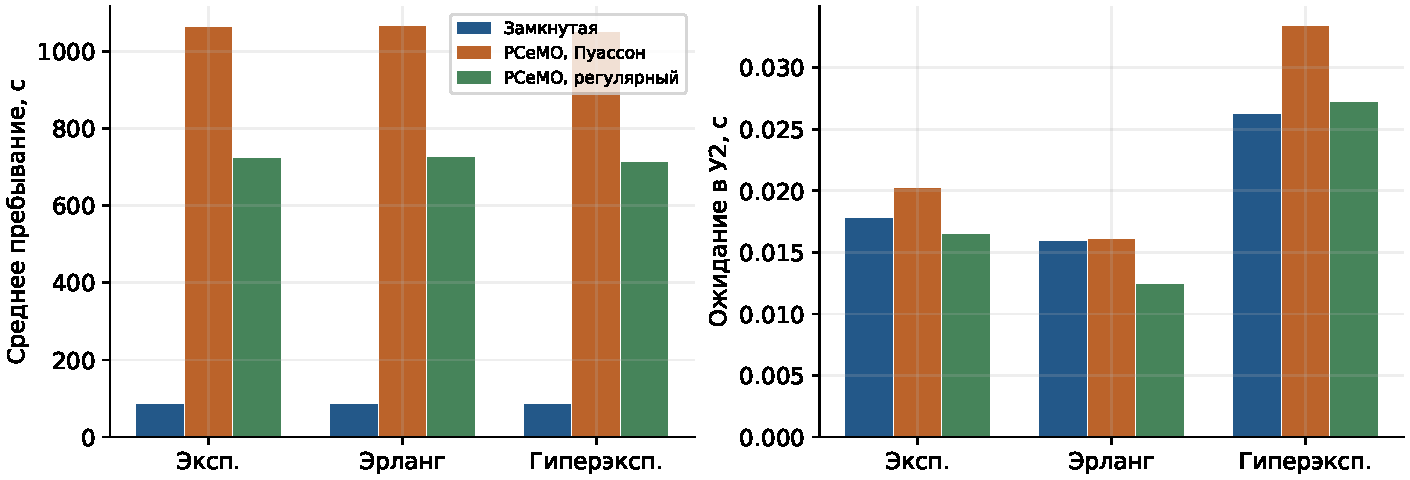
\includegraphics[width=\textwidth]{../out/part2/gpss/matched_service.pdf}
 \caption{Сравнение сетевого пребывания и ожидания в У2 при равном потоке}
 \label{fig:p2-match}
\end{figure}

\subsection{Распределения времени}

Для гистограмм на рисунке~\ref{fig:p2-native-hist} взяли частоты
из отчёта GPSS World по контрольному прогону замкнутой сети
при \(M=6\) (рисунок~\ref{fig:gp-network-report}).
За \(200\,000\) с измерения завершился
\(14\,221\) цикл. Среднее время цикла равно \(84{,}38\) с,
коэффициент вариации — \(1{,}30\). Аппроксимация \(H_2\)
по первым двум моментам даёт вероятность длинной компоненты
\(0{,}246\) и средние компонент \(171{,}56\) и \(55{,}94\) с.
На гистограмме много коротких циклов и заметен длинный правый
хвост. Параметры приближения подобраны по двум моментам, а саму
форму распределения показывает гистограмма.

Для пребывания в У2 коэффициент вариации \(0{,}98\)
близок к единице, что согласуется с экспоненциальной
аппроксимацией при базовом законе обслуживания. Ожидание
равно нулю в \(37{,}5\%\) циклов и \(98{,}6\%\) посещений
У2. Для аппроксимации ожидания эту вероятность выделяют
отдельно, а положительную часть описывают непрерывным
распределением. В разомкнутой сети высокие коэффициенты
вариации сетевого ожидания показывают, что существенная
часть разброса теряется при сравнении средних.

\begin{figure}[htbp]
 \centering
 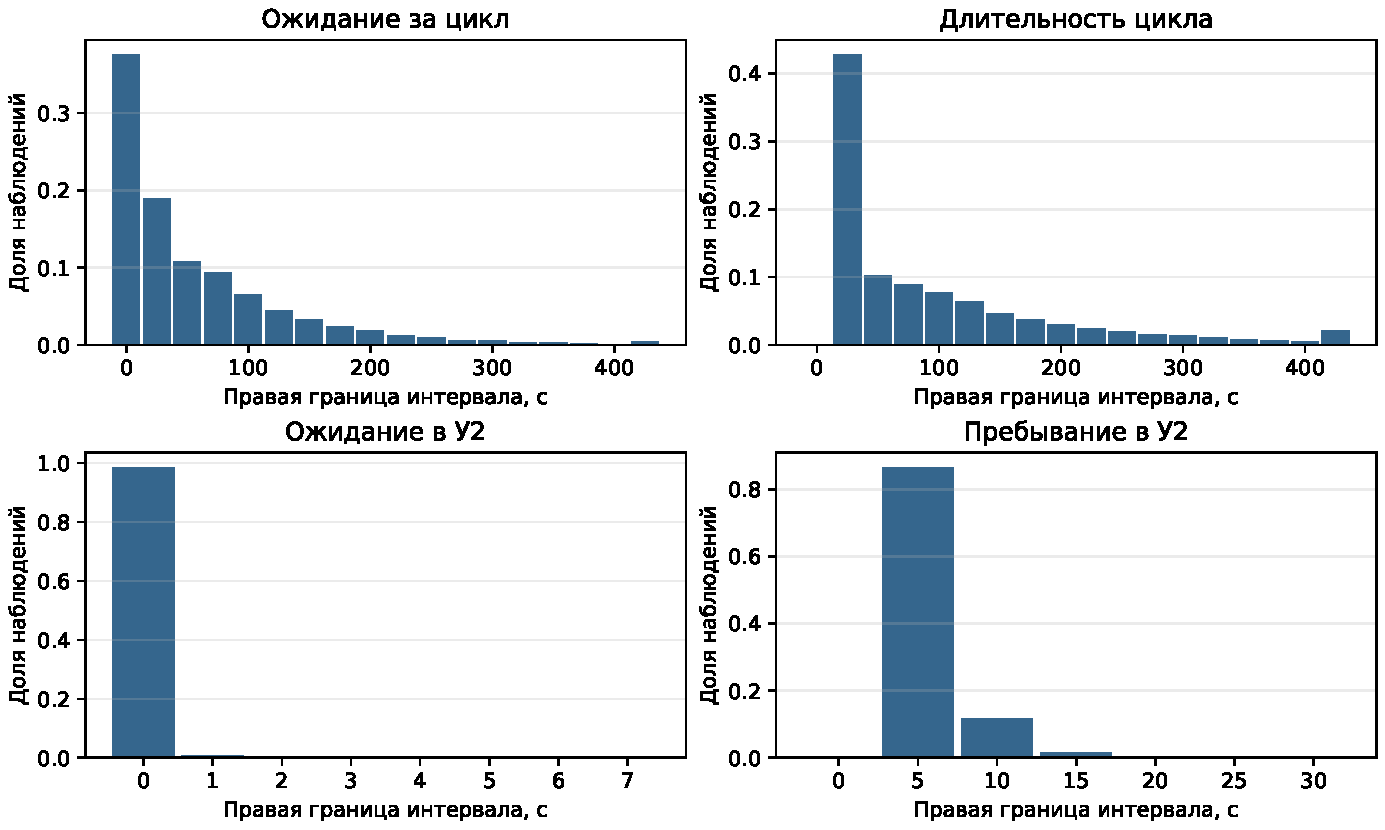
\includegraphics[width=.96\textwidth]{../out/part2/gpss_closed_histograms.pdf}
 \caption{Гистограммы сетевых и узловых времён из GPSS World.
 Замкнутая сеть, \(M=6\), экспоненциальное обслуживание}
 \label{fig:p2-native-hist}
\end{figure}

Для разомкнутой экспоненциальной сети при заданной
\(\rho_3=0{,}90\) контрольный прогон дал \(12\,634\) завершённых
заявки за \(200\,000\) с измерения. Среднее пребывание равно
\(120{,}06\) с при коэффициенте вариации \(1{,}62\).
Двухкомпонентная аппроксимация по моментам даёт вероятность
длинной компоненты \(0{,}166\) и средние \(362{,}23\)
и \(71{,}96\) с. В У2 коэффициент вариации пребывания
практически такой же, как в замкнутой сети (\(0{,}99\)).
Сетевое ожидание равно нулю в \(41{,}8\%\) наблюдений.
При этом длинные ожидания дают среднее \(83{,}23\) с.
Нулевая масса и длинный хвост видны одновременно на
сетевой гистограмме (рисунок~\ref{fig:p2-open-hist}).

\begin{figure}[htbp]
 \centering
 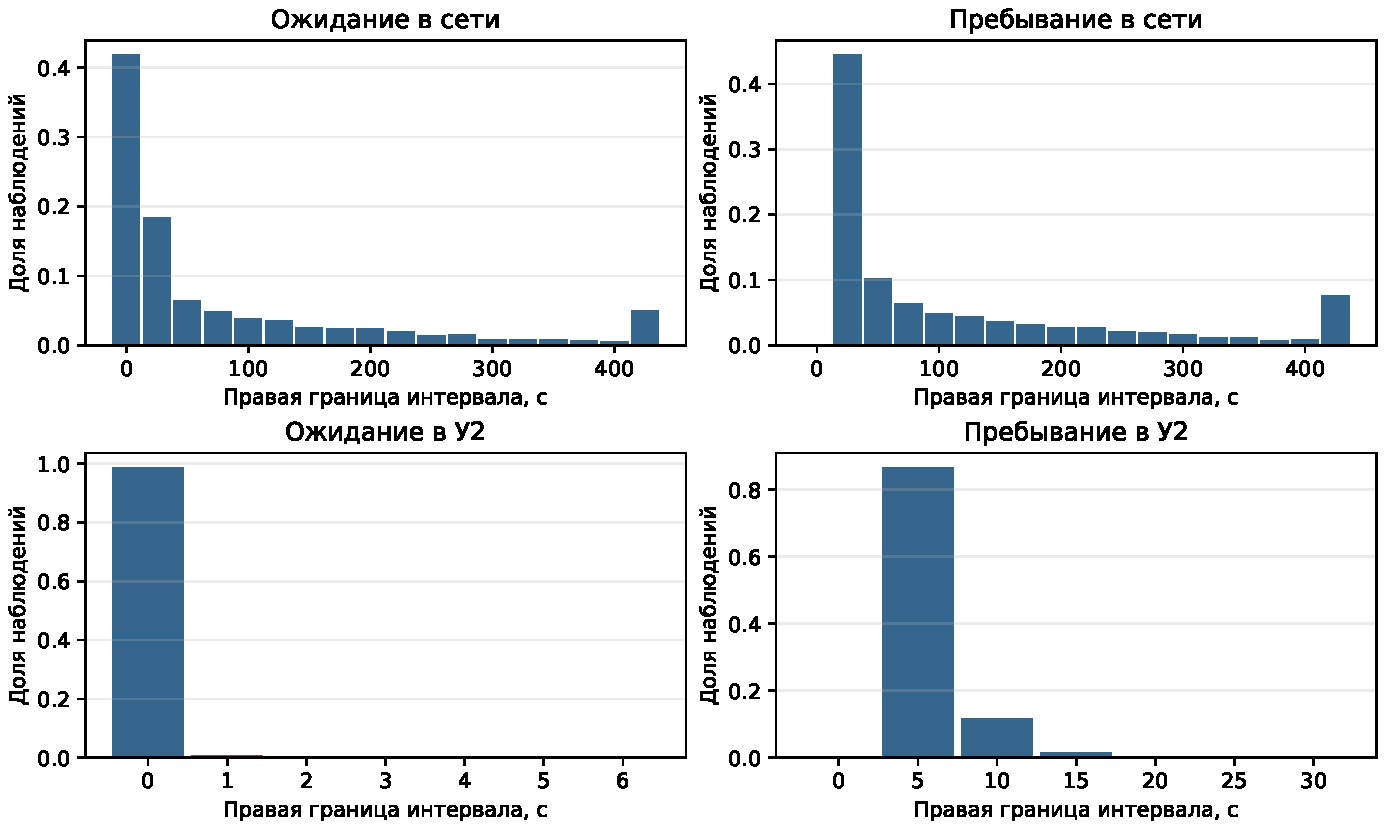
\includegraphics[width=.96\textwidth]{../out/part2/gpss_open_histograms.pdf}
 \caption{Гистограммы из GPSS World для разомкнутой сети с простейшим
 входом и экспоненциальным обслуживанием при заданной \(\rho_3=0{,}90\)}
 \label{fig:p2-open-hist}
\end{figure}
